\documentclass[11pt]{article}
\usepackage[hmargin=1in,vmargin=1in]{geometry}
\usepackage{xcolor}
\usepackage{amsmath,amssymb,amsfonts,url,sectsty,framed,tcolorbox,framed}
\newcommand{\pf}{{\bf Proof: }}
\newtheorem{theorem}{Theorem}
\newtheorem{lemma}{Lemma}
\newtheorem{proposition}{Proposition}
\newtheorem{definition}{Definition}
\newtheorem{remark}{Remark}
\newcommand{\qed}{\hfill \rule{2mm}{2mm}}
\newtheorem{example}{Example}
\usepackage{tikz}
\usepackage{bm}

\begin{document}
%%%%%%%%%%%%%%%%%%%%%%%%%%%%%%%%%%%%%%%%%%%%%%%%%%%%%%%%%%%%%%%%%%%%%
\noindent
\rule{\textwidth}{1pt}
\begin{center}
{\bf [CS304] Introduction to Cryptography and Network Security}
\end{center}
Course Instructor: Dr. Dibyendu Roy \hfill Winter 2023-2024\\
Scribed by: Raghav Agiwal (202151124) \hfill Lecture (Week 4)
\\
\rule{\textwidth}{1pt}
%%%%%%%%%%%%%%%%%%%%%%%%%%%%%%%%%%%%%%%%%%%%%%%%%%%%%%%%%%%
%write here
\section{Groups}

\textbf{Subgroup Conditions:}

\begin{itemize}
    \item \textit{Subset of $G$:} \\
    Confirm whether $H$ is a subset of the group $G$.
    
    \item \textit{Group Property:} \\
    Determine if $H$ constitutes a group under the operation $+$ of $G$.
\end{itemize}

\vspace{0.5cm}

\textbf{Definition:}

A subgroup $H$ of a group $(G, +)$ is defined as a non-empty subset that satisfies both conditions:
\begin{enumerate}
    \item $H$ is a subset of $G$.
    \item $H$ forms a group when equipped with the operation $+$ of $G$.
\end{enumerate}

If $H$ is a proper subset and a group of $G$, and $H$ is distinct from $G$, it is termed a proper subgroup of $(G, +)$.


\subsection{Group Properties}

\begin{itemize}
    \item \textbf{Closure Property:}
    \begin{itemize}
        \item In a group $(G, +)$, for any element $a$ belonging to $G$, it implies that adding $a$ to itself ($a + a$) results in another element that belongs to $G$. Similarly, adding $a$ four times ($a + a + a + a$) yields an element that also belongs to $G$.
    \end{itemize}
    
    \item \textbf{Notation:}
    \begin{itemize}
        \item We denote $a + a$ as $a^2$ and $a + a + a + a$ as $a^4$. Generally, for any positive integer $i$, $a^i$ represents the result of adding $a$ to itself $i$ times, which also belongs to $G$.
    \end{itemize}
    
    \item \textbf{Definition of Cyclic Group:}
    \begin{itemize}
        \item A group $G$ is termed cyclic if there exists an element $x$ within $G$ such that every element $b$ in $G$ can be expressed as $x$ raised to some power $i$, where $i$ is an integer.
    \end{itemize}
    
    \item \textbf{Generator:}
    \begin{itemize}
        \item The element $x$ that fulfills the condition above is called the generator of the group $(G, +)$.
    \end{itemize}
    
    \item \textbf{Order of an Element:}
    \begin{itemize}
        \item The order of an element $a$ in $G$, denoted as $O(a)$, is the smallest positive integer $m$ such that raising $a$ to the power $m$ results in the identity element $e$ of the group $G$.
    \end{itemize}
\end{itemize}



\subsection{Properties of Set $S$:}

Given $O(a) = 5$, where $a^5 = e$, and $S = \{e, a, a^2, a^3, a^4\}$.
We observe the following:
\begin{itemize}
    \item $a^4 + a = e$, which implies that the inverse of $a$ is $a^4$.
    \item $S$ is a subset of $G$.
\end{itemize}

\section{Proof that $(S, +)$ is a Group:}

\subsection{Subset of $G$:}

$S$ is a subset of $G$, meaning all elements of $S$ are also elements of $G$.

\subsection{Closure:}

For any $x, y \in S$, $x + y$ is also in $S$. For example, $a^2 + a^3 = a^5 = e$ which is in $S$.

\subsection{Associativity:}

The operation $+$ is associative since it is inherited from the group $G$. For any $x, y, z \in S$, $(x + y) + z = x + (y + z)$.

\subsection{Identity Element:}

The identity element $e$ exists in $S$. Any element $x$ combined with $e$ yields $x$. For instance, $a^2 + e = a^2$.

\subsection{Inverse Element:}

For each $x \in S$, there exists an inverse $y \in S$ such that $x + y = e$. For example, the inverse of $a^2$ is $a^3$ since $a^2 + a^3 = e$.

\subsection{Definition of Cyclic Subgroup:}

Let $G$ be a group and $a$ belongs to $G$.
The set of all powers of $a$ forms a cyclic subgroup generated by $a$, denoted by $\langle a \rangle$.
Mathematically, $\langle a \rangle = \{a^n | n \in \mathbb{Z}\}$.


\section{Lagrange's Theorem:}

If you have a finite group, let's call it \( G \), and inside that group, there's a smaller group called \( H \), which we call a subgroup, then the number of elements in \( H \), denoted as \( |H| \), divides the number of elements in \( G \), denoted as \( |G| \).

\subsection{Explanation:}

Lagrange's theorem is a critical concept in group theory. It tells us that when we have a subgroup of a finite group, the size of that subgroup must divide evenly into the size of the larger group. In simpler terms, if you have a group of certain size, any smaller group inside it must have a number of elements that "fits" perfectly into the larger group's total.

\subsection{Example:}

Let's say we have a group \( G \) with 12 elements. Now, imagine we find a subgroup \( H \) within \( G \) that has 3 elements. According to Lagrange's theorem, because \( H \) is a subgroup of \( G \), the number of elements in \( H \) must evenly divide the number of elements in \( G \). In this case, 3 does divide 12, so Lagrange's theorem holds true.

\subsection{Implications:}

\begin{itemize}
    \item Lagrange's theorem is incredibly useful for understanding the structure of finite groups.
    \item It helps us classify groups and grasp their internal workings.
    \item This theorem has practical applications in cryptography, coding theory, and various other mathematical fields.
\end{itemize}


\section{Ring:}

A ring \( (R, +_r, \cdot_r) \) is a mathematical structure consisting of a set \( R \) equipped with two binary operations: addition \( +_r \) and multiplication \( \cdot_r \).

\subsection{Properties of a Ring:}

\subsubsection{Abelian Group:}

The addition operation \( +_r \) on the set \( R \) forms an abelian (commutative) group.

\textbf{Example:} Consider the set of integers \( \mathbb{Z} \). Addition of integers is commutative, i.e., \( a + b = b + a \).

\subsubsection{Associativity:}

The multiplication operation \( \cdot_r \) is associative.

\textbf{Example:} In the set of real numbers \( \mathbb{R} \), multiplication is associative, i.e., \( (a \cdot b) \cdot c = a \cdot (b \cdot c) \).

\subsubsection{Multiplicative Identity:}

There exists a multiplicative identity element \( 1_r \) such that \( 1_r \cdot_r a = a \cdot_r 1_r = a \) for all \( a \) in \( R \).

\textbf{Example:} In the set of integers \( \mathbb{Z} \), the multiplicative identity is 1 since \( 1 \cdot a = a \cdot 1 = a \) for any integer \( a \).

\subsection{Distributivity:}

The multiplication operation \( \cdot_r \) distributes over addition \( +_r \).

\textbf{Example:} In the set of real numbers \( \mathbb{R} \), multiplication distributes over addition, i.e., \( (b + c) \cdot a = (b \cdot a) + (c \cdot a) \).

\textbf{Zero Divisors:}

In a ring, there may exist elements \( a \) and \( b \) such that \( a \cdot b = 0 \), where neither \( a \) nor \( b \) is zero. These elements are called zero divisors.

\subsubsection{Commutative Ring:}

A commutative ring \( (R, +_r, \cdot_r) \) is a type of ring where the multiplication operation \( \cdot_r \) satisfies the commutative property. In other words, for all elements \( a, b \) in \( R \), \( a \cdot_r b = b \cdot_r a \).

\subsubsubssection{Example:}

An example of a commutative ring is the set of integers \( \mathbb{Z} \) with the usual addition and multiplication operations. In \( \mathbb{Z} \), multiplication of integers is commutative, i.e., \( a \cdot b = b \cdot a \) for any integers \( a \) and \( b \).

\subsubsection{Unit or Invertible Element:}

An element \( a \) of a ring \( R \) is called a unit or invertible element if there exists another element \( b \) in \( R \) such that \( a \cdot_r b = 1_r \), where \( 1_r \) is the multiplicative identity element of \( R \).

\textbf{Example of Unit Element:}

In the ring of integers \( \mathbb{Z} \), the units are \( 1 \) and \( -1 \), since \( 1 \cdot 1 = 1 \) and \( (-1) \cdot (-1) = 1 \).

\subsubsection{Group of Units:}

The set of units in a ring \( R \) forms a group under the multiplicative operation \( \cdot_r \). This group is known as the group of units of \( R \).


\textbf{Properties of Group of Units:}
\begin{itemize}
    \item The group of units is closed under multiplication and contains the multiplicative identity element.
    \item Each element in the group of units has a multiplicative inverse within the group.
    \item The group of units is associative and satisfies the identity property.
\end{itemize}

\textbf{Example of Group of Units:}
In the ring of integers \( \mathbb{Z} \), the group of units is \( \{1, -1\} \), as these are the only elements with multiplicative inverses (their own inverses).


\section{Field}

\textbf{Definition of a Field:}

A field, denoted as \( F \), consists of a collection of elements. It has two main operations: addition (+) and multiplication (\( \ast \)). For a set to be considered a field, it must satisfy several properties:

\begin{enumerate}
    \item The addition operation must form a commutative group. This means that adding any two elements from the set should give the same result regardless of the order in which they are added. Additionally, there must be an identity element (usually denoted as \( 0_F \)) such that adding it to any element doesn't change the element.
    
    \item Excluding the additive identity, the nonzero elements in the set, when considered with the multiplication operation, should form an abelian group. This means that multiplying any two nonzero elements should also yield a nonzero element, and there should be an identity element for multiplication (usually denoted as \( 1_F \)) such that multiplying it with any element doesn't change the element.
    
    \item The distributive property must hold. This property states that for any three elements \( a, b, c \) in the set, the product of \( a \) with the sum of \( b \) and \( c \) is equal to the sum of the products of \( a \) with \( b \) and \( a \) with \( c \).
\end{enumerate}


\subsection{Field Extension}

In mathematics, a field extension occurs when we have two fields, let's call them \( K_1 \) and \( K_2 \), where \( K_2 \) contains all the elements of \( K_1 \) along with some additional elements.

\textbf{Explanation:}

Let's say we have a field \( K_2 \) with two operations, addition (+) and multiplication (\(\ast\)). Now, consider a subset \( K_1 \) of \( K_2 \) that is closed under both addition and multiplication, meaning that when we perform addition or multiplication on any two elements of \( K_1 \), the result remains within \( K_1 \). If \( K_1 \) itself is a field under the restrictions of addition and multiplication inherited from \( K_2 \), then \( K_1 \) is termed a subfield of \( K_2 \). Consequently, \( K_2 \) is called a field extension of \( K_1 \).

\textbf{Example:}

Consider the field of real numbers \( \mathbb{R} \) and the field of complex numbers \( \mathbb{C} \).
\begin{itemize}
    \item \( \mathbb{R} \) is a subset of \( \mathbb{C} \) since every real number is also a complex number with zero imaginary part.
    \item Both \( \mathbb{R} \) and \( \mathbb{C} \) satisfy the properties of a field, including closure under addition and multiplication, existence of additive and multiplicative identities, and existence of additive and multiplicative inverses.
    \item Therefore, \( \mathbb{R} \) is a subfield of \( \mathbb{C} \), and \( \mathbb{C} \) is a field extension of \( \mathbb{R} \).
\end{itemize}

\subsection{Polynomial Ring}

A polynomial ring is a fundamental algebraic structure that arises from the combination of a field and polynomials. Here's an explanation along with an example:\\

\textbf{Polynomial Ring:}

Let \( \mathbb{F} \) be a field, denoted as \( (\mathbb{F}, +, \ast) \). The polynomial ring \( \mathbb{F}[x] \) is defined as the set of all polynomials with coefficients from the field \( \mathbb{F} \).

\textbf{Explanation:}

In simple terms, the polynomial ring \( \mathbb{F}[x] \) consists of all polynomials where the coefficients come from the field \( \mathbb{F} \). A polynomial is an expression that involves variables raised to powers and multiplied by coefficients.

\textbf{Example:}

Consider the field of real numbers \( \mathbb{R} \). The polynomial ring \( \mathbb{R}[x] \) consists of all polynomials with real number coefficients. Here's an example of a polynomial in \( \mathbb{R}[x] \):

\[ f(x) = 3x^2 + 2x - 1 \]

In this polynomial:
\begin{itemize}
    \item \( 3 \), \( 2 \), and \( -1 \) are coefficients belonging to \( \mathbb{R} \).
    \item \( x \) is the variable.
    \item \( x^2 \), \( x \), and \( 1 \) are the monomials (terms) with corresponding coefficients.
\end{itemize}
This polynomial belongs to the polynomial ring \( \mathbb{R}[x] \) since all coefficients (\( 3 \), \( 2 \), and \( -1 \)) are real numbers.

The polynomial ring \( \mathbb{R}[x] \) contains infinitely many polynomials with different coefficients, powers, and combinations of terms, making it a powerful mathematical tool in algebra and other areas of mathematics.

\subsubsection{Addition Operation in Polynomial Ring:}

In the polynomial ring $F[x]$, addition of two polynomials $a(x)$ and $b(x)$ involves adding corresponding coefficients. Let's consider polynomials:

\[
a(x) = a_0 + a_1x + a_2x^2 + \ldots + a_{n-1}x^{n-1}
\]
\[
b(x) = b_0 + b_1x + b_2x^2 + \ldots + b_{n-1}x^{n-1}
\]

where $a_i$ and $b_i$ are coefficients belonging to the field $F$ for $0 \leq i < n$.

The addition operation of polynomials $a(x)$ and $b(x)$ in $F[x]$ results in a polynomial $c(x)$ given by:

\[
c(x) = (a_0 + b_0) + (a_1 + b_1)x + (a_2 + b_2)x^2 + \ldots + (a_{n-1} + b_{n-1})x^{n-1}
\]

where $a_i + b_i$ represents the addition operation in the field $F$.

\textbf{Example:}

Consider two polynomials in $\mathbb{R}[x]$:
\[
a(x) = 2x^2 + 3x + 1
\]
\[
b(x) = x^2 - 2x + 5
\]

The addition of these polynomials yields:
\[
c(x) = (2 + 1)x^2 + (3 - 2)x + (1 + 5)
\]
\[
c(x) = 3x^2 + x + 6
\]

\subsubsection{Multiplication Operation in Polynomial Ring:}

Similar to addition, multiplication of two polynomials $a(x)$ and $b(x)$ in $F[x]$ involves multiplying corresponding coefficients. Using the same polynomials as above:

\[
a(x) = a_0 + a_1x + a_2x^2 + \ldots + a_{n-1}x^{n-1}
\]
\[
b(x) = b_0 + b_1x + b_2x^2 + \ldots + b_{n-1}x^{n-1}
\]

The multiplication operation of polynomials $a(x)$ and $b(x)$ in $F[x]$ results in a polynomial $c(x)$ given by:

\[
c(x) = (a_0 \cdot b_0) + (a_1 \cdot b_1)x + (a_2 \cdot b_2)x^2 + \ldots + (a_{n-1} \cdot b_{n-1})x^{n-1}
\]

where $a_i \cdot b_i$ represents the multiplication operation in the field $F$.

\textbf{Example:}

Using the same polynomials as before:
\[
a(x) = 2x^2 + 3x + 1
\]
\[
b(x) = x^2 - 2x + 5
\]

The multiplication of these polynomials yields:
\[
c(x) = (2 \cdot 1)x^4 + (2 \cdot (-2) + 3 \cdot 1)x^3 + \ldots + (1 \cdot 5)
\]
\[
c(x) = 2x^4 + (-4 + 3)x^3 + \ldots + 5
\]


\noindent \textbf{Irreducible Polynomial:}

An irreducible polynomial in a given field is a polynomial that cannot be factored into the product of two non-constant polynomials over that field. In simpler terms, it's a polynomial that cannot be broken down into simpler components.

\vspace{5mm}

\textbf{Example:}
\begin{itemize}
    \item In the polynomial ring of real numbers, the polynomial $x^2 + 1$ is irreducible because it cannot be factored into polynomials of lower degree over the real numbers.
\end{itemize}

\vspace{5mm}

\textbf{Characteristics:}
\begin{itemize}
    \item \textbf{Degree:} Irreducible polynomials typically have a degree greater than 1.
    \item \textbf{Indivisibility:} They cannot be divided evenly by any other non-constant polynomials in the same field.
    \item \textbf{Unique Factorization:} If a polynomial can be factored, its factorization is unique up to the order of the factors and multiplication by units of the field.
    \item \textbf{Applications:} Irreducible polynomials are fundamental in various areas of mathematics, including number theory, algebraic geometry, and cryptography.
\end{itemize}

\vspace{5mm}

\textbf{Ideal $I = \langle p(x) \rangle$:}

The ideal generated by an irreducible polynomial $p(x)$ consists of all polynomials that are multiples of $p(x)$. It's denoted as $I = \langle p(x) \rangle$.

\vspace{5mm}

\textbf{Division in Quotient Ring $F[x]/\langle p(x) \rangle$:}

When dividing a polynomial $q(x)$ by an irreducible polynomial $p(x)$, we obtain a quotient polynomial $d(x)$ and a remainder polynomial $r(x)$, both belonging to the quotient ring $F[x]/\langle p(x) \rangle$. This process is analogous to division with integers, but it operates within the context of polynomials and modulo arithmetic.

\vspace{5mm}

\textbf{Further Examples:}
\begin{enumerate}
    \item In the field of rational numbers, the polynomial $x^2 - 2$ is irreducible because it cannot be factored into linear factors with rational coefficients.
    \item Over the field of integers modulo $5$, the polynomial $x^2 + x + 1$ is irreducible because it does not have any roots in $\mathbb{Z}_5$.
\end{enumerate}



\section*{AES - Advanced Encryption Standard}

AES stands for Advanced Encryption Standard. It's a widely used symmetric encryption algorithm that ensures secure communication and data protection. AES was established as a standard by the U.S. National Institute of Standards and Technology (NIST) in 2001 and has since become one of the most commonly used encryption methods worldwide.

AES operates on fixed-size blocks of data and uses a fixed-length key for encryption and decryption. It supports key sizes of 128, 192, and 256 bits. The number in AES (e.g., AES-128, AES-192, AES-256) refers to the key size in bits.

\subsection*{Key Sizes}

\begin{itemize}
    \item \textbf{AES-128}: Uses a 128-bit key for encryption and decryption. Operates on data blocks of 128 bits and performs 10 rounds of encryption for a given key.
    \item \textbf{AES-192}: Uses a 192-bit key for encryption and decryption. Operates on data blocks of 128 bits and performs 12 rounds of encryption for a given key.
    \item \textbf{AES-256}: Employs a 256-bit key for encryption and decryption. Similar to AES-128, it operates on data blocks of 128 bits but performs 14 rounds of encryption for a given key.
\end{itemize}

\begin{figure}[htbp]
  \centering
  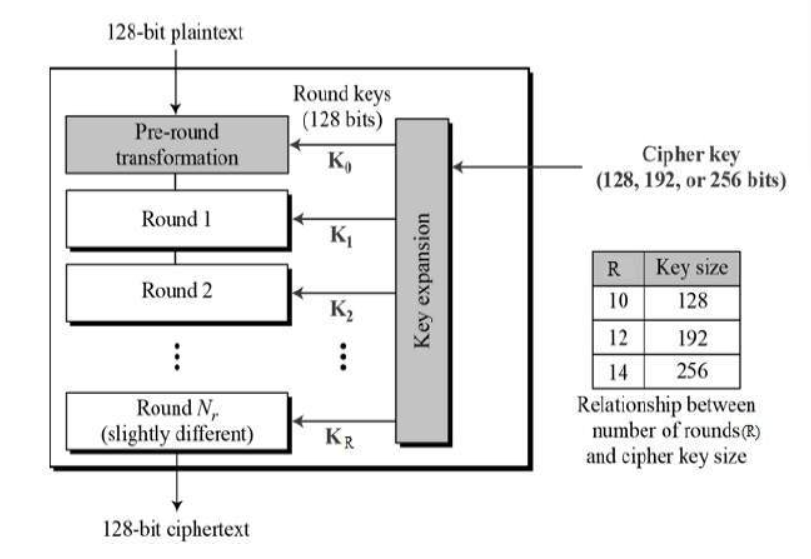
\includegraphics[width=1.00\textwidth]{image4.1.PNG} % Replace example-image with your image file
\end{figure}



\end{document}